\section{Introduction}
Agilefant is an open source tool for task and requirement management for agile 
software development. It is provided as an open-source version and a hosted 
version. The hosted version comprises more and better features in comparison to 
the open-source version.

Agilefant has approximately 10,000 users worldwide, and according to the 
customer, the number of registered users increases every day. 
 
Agilefant is a very powerful tool for requirement management but currently it 
is too detailed to be used on mobile devices (small screens). The customer 
wishes that the users of Agilefant could use its the most important functions 
using their mobile phones and tablets. Agilefant's main competitors are already 
providing mobile applications, so it is crucial to Agilefant to response for 
this. Therefore, the goal of our team is to develop a mobile application that 
works along the hosted version of Agilefant and can be used on both smart 
phones and tables.

\section{Stakeholders and staffing}

The group's web page is located in 
\href{https://studentwiki.aalto.fi/display/MOB/Mobilefant+Home}{Studentwiki}. 

The group's email is mobilefant\#agilefant.org.

\subsection{The Team}

Here we are only listing the role, name, email, responsibilities and an 
assistant role of each team member. We have a document with everyone's personal 
informations such as email, phone number and Github name, but we won't publish 
those informations excluding email.

\begin{table}[H]
\center
\begin{adjustwidth}{-1cm}{}
\begin{tabular}{|p{1.8cm}|p{3cm}|p{4.1cm}|p{4.1cm}|p{1.8cm}|} 
	
\hline % The line on top of the table
\textbf{Role} & \textbf{Name} & \textbf{Email} & \textbf{Responsibilities} & 
\textbf{Assistant role} \\ 
\hline 
Project Manager & Benjamin Behm & benjamin.behm\#aalto.fi & Organizing the 
work, removing impediments, documenting, process supervising, coding & - \\ 
\hline
Architect & Harri Lampi & harri.lampi\#aalto.fi & Architectural design & - \\ 
\hline
Quality Assurance & Matias Kuusela & matias.kuusela\#aalto.fi & QA & - \\ 
\hline
Developer & Aleksi Hoffman & aleksi.hoffman\#aalto.fi & & \\
\hline
Developer & Miro Vilkki & miro.vilkki\#aalto.fi &  & \\
\hline
Developer & Rolle Saarinen & rolle.saarinen\#aalto.fi &  & \\
\hline
Developer & Janne Gröndahl & janne.grondahl\#aalto.fi & & \\
\hline
Developer & Janne Kajovuori & janne.kajovuori\#aalto.fi & & \\
\hline
Developer & Joakim Kronqvist & joakim.kronqvist\#aalto.fi & & \\
\hline

\end{tabular} % for really simple tables, you can just use tabular
\end{adjustwidth}
\caption{The team}
\label{table:Team}
\end{table}

NB! Each developer should act as an assistant to some of the SE experts in 
order to get a broader view to the project.


\subsection{Mentor}

\begin{table}[H]
\center
\begin{tabular}{|p{2cm}|p{3.8cm}|p{4.1cm}|} 

\hline 
\textbf{Role} & \textbf{Name} & \textbf{Email} \\ 
\hline
Mentor & Casper Lassenius & casper.lassenius\#aalto.fi \\
\hline
\end{tabular}
\caption{Mentor}
\label{table:Mentor}
\end{table}

\subsection{Customer}

\begin{table}[H]
\center
\begin{tabular}{|p{2cm}|p{3.8cm}|p{4.1cm}|} 
	
\hline 
\textbf{Role} & \textbf{Name} & \textbf{Email}\\ 
\hline
Product owner & Jarno Vähäniitty & jarno\#agilefant.org\\
\hline
Tech. Lead & Santeri Korri & santeri\#agilefant.org\\
\hline
\end{tabular} 
\caption{Customer representatives}
\label{table:Customer}
\end{table}



\section{The Goals}
\subsection{Project goals}

The main goal is to develop a mobile application for Agilefant that contains 
the main functionalities of its cloud version.

\begin{table}[H]
\center
\begin{tabular}{|p{0.5cm}|p{6.5cm}|p{6.5cm}|} 

\hline 
\centering \textbf{\#} & \textbf{Goal} & \textbf{Verification Criteria} \\ 
\hline
\centering 1 & To build a limited set of key use cases & Architecturally sound, 
clear implementation and testable \\
\hline
\centering 2 & - & - \\
\hline
\end{tabular}
\caption{Project goals in the priority order}
\label{table:Projectgoals}
\end{table}


\subsection{Personal goals}

Personal learning goals can be found in Google Docs: 
\href{https://docs.google.com/spreadsheet/ccc?key=0Ahu59q_GwtcedHJZdjQ1RWROZFYxa
0RTcWp3MkJkTnc&usp=sharing}{Learning Goals}

\section{Resources}
\subsection{Personnel}

Each member must invest credits * 27 hours - 15 hours in the project.

\href{https://docs.google.com/spreadsheet/ccc?key=0Ahu59q_GwtcedHI3MnJQM0NWZS11a
GxFTzFZeVEyQVE&usp=sharing}{Link} to the time allocation page. Everyone should 
mark how much time he/she is going to use per a week to the table.

\subsection{Material}

We need mobile phones to test the application. The customer has promised to 
deliver some test phones, but a wide range of different phones with different 
platforms cannot be guaranteed. The CSE department can borrow desktop computers 
to our group with virtual machines installed. These computers need to be set up 
to our team room A243.

The room (A243) will be shared with an another project group (\#15 - 
TrafficSense) so we need to schedule the usage of the room with them. The idea 
will be that both teams will have specific days and hours the room is 
exclusively reserved for them. At other times, everyone could use the room.

A development environment can be downloaded from Internet if needed. Eclipse is 
an open-source and free to download, and the project manager has a JetBrain's 
Classroom License, so that IntelliJ IDEA Ultimate can be used during the course.

\section{Work practices}
\subsection{Practices}
\subsubsection{Iterative development}

Development will be divided into several sprints so that after every sprint we 
would have an improved product increment of the application ready to release. 

A sprint contains four phases: sprint planning, development, demo, and 
retrospective. 

\begin{figure}[H]
\centering
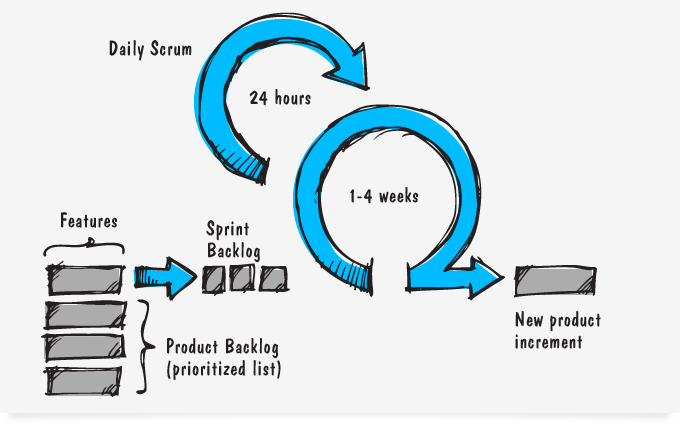
\includegraphics[width=1\textwidth]{imgs/scrum_process_en.png}
\caption{Scrum process}
\label{fig:scrum}
\end{figure}

\subsubsection{Sprint planning}

Sprint planning session will be divided into two parts. The content of the 
sprint planning is presented in Table~\ref{table:Sprintplanning}.

Stories will be estimated based on fibonacci numbers.
Story points will be given based on people’s opinion of how much time it 
requires to finish the story. Possible story points are listed below:
\begin{description*}
\item[1:] without a break
\item[2:] half a day
\item[3:] a day (= full work day for a pair)
\item[5:] two work days
\item[10:] five days
\end{description*}
	
If the story is estimated to be larger than 10 story points, it can be seen as 
an epic and should be split to smaller stories so that it can be finished 
during the sprint.


\begin{table}[H]
\center
\begin{tabular}{|p{1cm}|p{2cm}|p{5cm}|p{4cm}|} 
	
\hline 
\textbf{Part} & \textbf{Duration} & \textbf{Description} & 
\textbf{Participants} \\ 
\hline
1 & 1h & The product owner presents the prioritized product backlog, so that 
the teams would understand what should be done during a following sprint. The 
product owner is there for answering any questions the teams would like to ask 
relating to the user stories and tasks. Then the teams select items from the 
product backlog to the sprint backlog based on their knowledge of how much work 
they are capable of doing during a sprint. Sprint goal is agreed in this part. 
& Product owner, team members \\
\hline
2 & 2h & Teams are separated to plan how the chosen work will be done during 
the sprint. Users stories will be assigned to team members. User stories are 
split into tasks and the required time per a task is estimated by a person the 
task was assigned to. In this meeting, the team can start design the system so 
that they are able to convert the backlog items into a working software 
increment. & Team members \\
\hline
\end{tabular} 
\caption{The content of a sprint planning}
\label{table:Sprintplanning}
\end{table}

\subsubsection{Documenting}

\subsubsection{Risk management}

\subsubsection{Time tracking}

The groups' time tracking will be applied in Agilefant. The group should follow these time tracking practices:
\begin{itemize}
\item Each group member should enter their own hours by themselves to the Agilefant.
\item Hours are logged directly to the story or more preferably to the task after the work is done. 
\item Hours should be logged before leaving the office
\end{itemize}

Agilefant provides burndown charts that are used to follow the project's progress and those also tell whether estimated hours are correlating with actual hours. That helps group to shape its task estimation.

As the group is logging spent effort to the Agilefant, the customer is able to follow whether the group is working as promised. 

\begin{figure}[H]
\centering
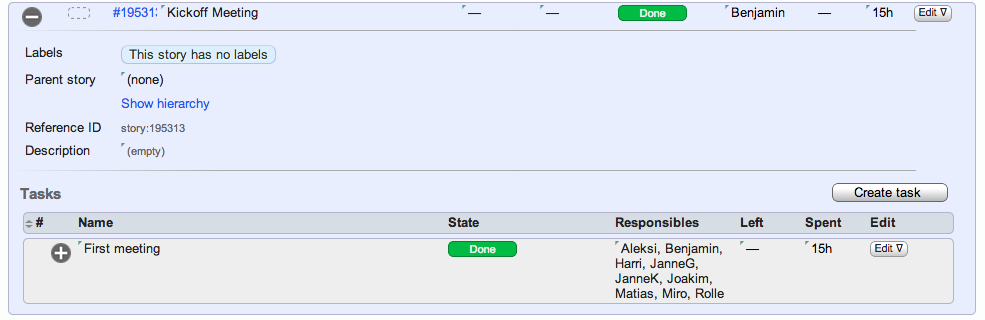
\includegraphics[width=1\textwidth]{imgs/spenteffort1.png}
\caption{Story and task with spent effort}
\label{fig:spenteffort1}
\end{figure}


\begin{figure}[H]
\centering
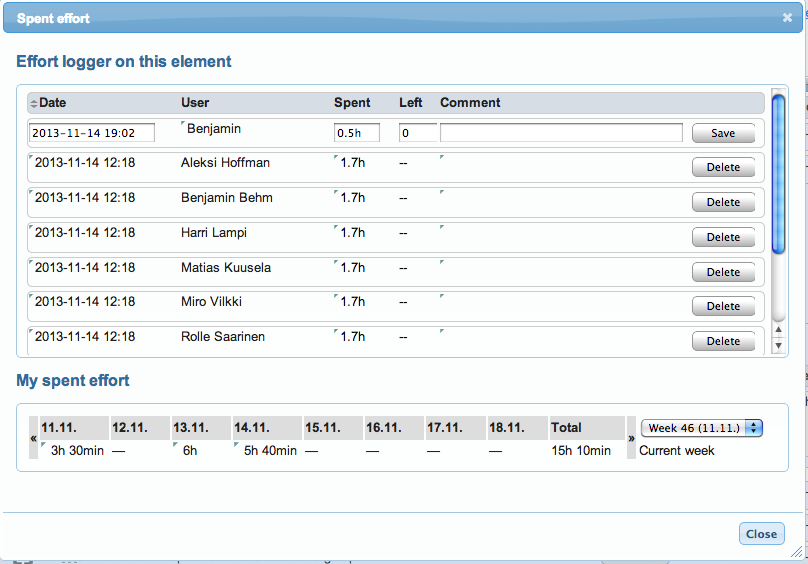
\includegraphics[width=1\textwidth]{imgs/spenteffort2.png}
\caption{Log spent effort}
\label{fig:spenteffort2}
\end{figure}

When the course is over, credits will be given based on the hours logged to the 
Agilefant (+ hours spent on lectures). The view shown in 
Figure~\ref{fig:totalhours} can be found in Timesheets where user needs to 
select backlog(s), interval and user(s) to generate the timesheet where used 
hours are listed.

\begin{figure}[H]
\centering
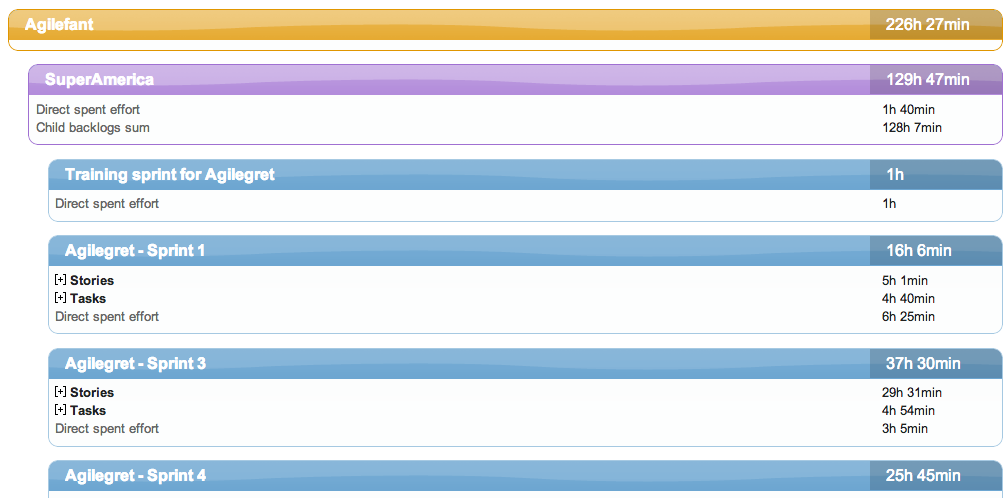
\includegraphics[width=1\textwidth]{imgs/totalhours.png}
\caption{Total used hours}
\label{fig:totalhours}
\end{figure}

\subsubsection{Communication}

Team will keep a daily standup meeting every time they gather together to work. 
The daily standup will be a short, 15-minute time-boxed meeting where team 
members synchronize their activities. In this meeting, people will tell, in 
turn, three things: What they have done since last daily meeting, what they 
will do before the next meeting, and what obstacles are in the way.  

The product manager will propose if the team could use Flowdock as the main 
communication tool. Aalto provides 180 days license for that.

Google Hangout is proposed to be used for communication with off-site team 
members.

In very urgent situations phone calls or text messaging can be used, but primary the group is using tools mentioned above.

\subsubsection{Defect tracking}

Agilefant could be used

\subsubsection{Version control}

Git and Github will be used for version control. 

TODO: How to use it when 3 teams? Check options from 
\href{https://www.atlassian.com/git/workflows}{here}.

\subsubsection{Process improvement}

A retro will be arranged at the end of each sprint. There will be three phases:

\begin{enumerate}
\item First, we will go through impediments from the previous retro and check 
if the impediments has been fixed.
\item Second, each team member will write down aspects that has worked well and 
which might need some attention.
\item Third, these will be collected and written to Excel and everyone should 
explain what they wrote.
\end{enumerate}

\subsubsection{Requirement engineering}

Agilefant will be used for gathering requirements from customer and maintaining 
the backlog. 

\subsubsection{Design}

\subsubsection{Practice X}

\section{Phasing}

Tasks are not listed in this project plan, as they are listed and maintained in 
\href{https://cloud.agilefant.com/dev/}{Agilefant}.

\subsection{Schedule}



\subsection{Sprint 1 Plan}

Goals:
\begin{itemize}
\item To understand Agilefant's vision
\item To have the main requirements from the Customer
\item To understand the process that is used in the course
\item To have a draft of the architecture design
\end{itemize}

\subsection{Sprint 2 Plan}

Goals:
\begin{itemize}
\item Set up the development environment
\item Get touch with the code 
\item To have the code base ready 
\item To have the architecture design ready
\end{itemize}

\noindent Deliverables:
\begin{itemize}
\item Project plan (no QA plan)
\item Progress report slides
\item Contract (one per group)
\item Requirements document (except details of requirements)
\end{itemize}

\section{Risk log}

\begin{table}[H]
\center
\begin{adjustwidth}{-2cm}{}
\begin{tabular}{|p{0.5cm}|p{3cm}|p{1cm}|p{1.5cm}|p{3cm}|p{3cm}|p{3cm}|} 
	
\hline % The line on top of the table
\textbf{ID} & \textbf{Risk} & \textbf{Prob.} & \textbf{Sev.} & \textbf{Effects} 
& \textbf{Controlling actions} & \textbf{Responsible} \\ 
\hline
1 &
A developer quits in the middle of the project.
2 &
3 &
Some knowledge is lost. &
Project scope must be decreased. &
Taking care of good team spirit.
Using pair programming. &
The team / project manager \\
\hline
\end{tabular} 
\caption{A risk log (Probability: 1=lowest, 3=highest, Severity: 1= lowest, 
3=highest)}
\label{table:Risklog}
\end{adjustwidth}
\end{table}
